% !TEX TS-program = pdflatexmk
\documentclass[11pt]{article}
\usepackage[margin=.8in]{geometry}
\usepackage{amsmath,amssymb,amsthm, latexsym, mathrsfs, pdfsync, multicol,
fancybox, fancyhdr,
graphicx, enumerate,
subfig, tikz, pgfplots,array}

%\singlespacing
\def\RR{{\mathbb R}}
\def\NN{{\mathbb N}}
\def\ZZ{{\mathbb Z}}
\def\QQ{{\mathbb Q}}
\def\CC{{\mathbb C}}
\def\bc{\begin{center}}
\def\ec{\end{center}}
\def\be{\begin{enumerate}}
\def\ee{\end{enumerate}}
\def\bi{\begin{itemize}}
\def\ei{\end{itemize}}
\def\t{\times}
\newcommand{\ol}[1]{\overline{#1}}
\newcommand{\oimp}[1]{\overset{#1}{\Longleftrightarrow}}
\newcommand{\bv}[1]{\ensuremath{ \mathbf{\vec{#1}}} }
\renewcommand{\d}{\displaystyle}
\newcommand{\blank}[1]{\rule{#1}{0.75pt}}

\usetikzlibrary{calc}

\lhead{\sc{Math 316 Hist. of Math.}}
\chead{\large \sc Midterm II} 
\rhead{\sc Spring 2023}
\cfoot{}
\pagestyle{fancy}
%
\begin{document}
\thispagestyle{fancy}

\vspace{1in}

\textbf{Student Name:} Solutions

\vspace{1in}



\bc Part I \ec

This part is written without notes or aids of any kind. It is worth 27 points out of 100 total points. \\

Below is a list of nine mathematicians, listed in alphabetical order. For each name, state whether the he lived before or after Euclid. Next to each name, state the title of a mathematical work the person authored \textbf{OR} a mathematical theorem or idea for which this person is given credit.\\

There are many many correct answers for each mathematician.

\be
\item Archimedes (order: after) Quadrature of the Parabola
\item Apollonius of Perga (order: after) \textit{Conics}
\item Eratosthenes (order: after) Estimation of the circumference of Earth
\item Eudoxus of Cnidos (order: before) Theory of proportions used by Euclid in \textit{Elements}


\item Hippias of Elis (order: before) Construction of the Quadratrix and its use in trisecting an angle

\item Hippocrates of Chios (order: before) Quadrature of a Lune
\item Claudius Ptolemy (order:after) \textit{Almagest}
\item Thales of Miletos (order: before) Vertical angles are equal.
\item Zeno of Elia (order: before) Framing several paradoxes including one about the tortoise and Achilles.

\ee
\bc Part II \ec

For this part, you may use a calculator and up to two pages of notes. This part is worth 73 points out of 100 total points. All parts of all questions are either mathematical or \textbf{short answer.} Short answer questions do not require more than an appropriately detailed sentence or two.

\be
%%%quadratrix
\item (13 points) The questions below concern Hippias' development of the Quatratrix. The figure of the quadratrix (below) is from our textbook. Recall that the thick arc from B through F to G is the curve.
\begin{center}
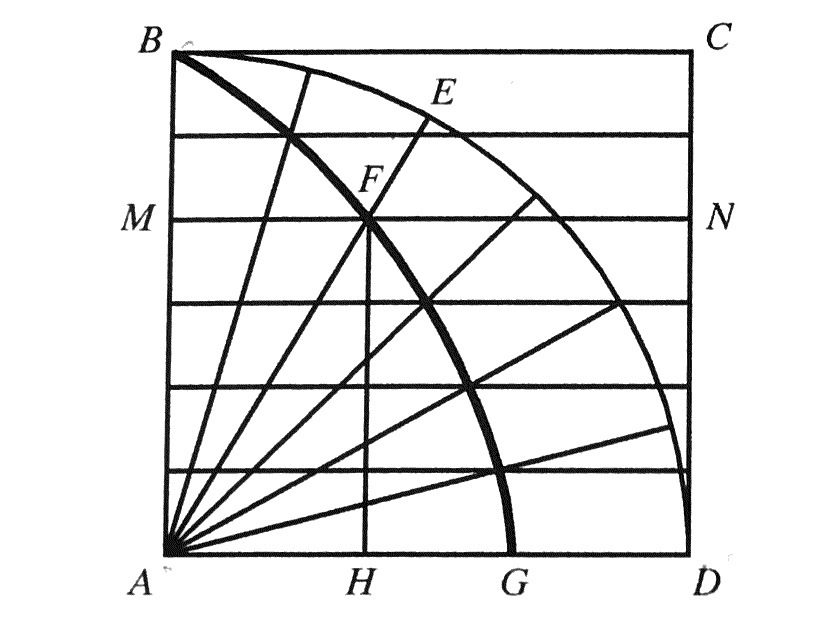
\includegraphics[scale=0.25]{quadratrix.jpg}
\end{center}
	\begin{enumerate}
	\item Give a precise mathematical relationship between $\angle EAD$ and line segment $FH.$ 
	
	$\frac{\angle EAD}{\angle BAD} = \frac{BA}{FH}$ 
	
	\item Explain why Hippias' definition of the quadratrix technically did not contain point $G$ and explain how we define that point in modern terms.\\
	In his definition, points were determined by the intersection of two lines and those lines coincide along $AD.$
	\item Hippias' used the quadratrix for what purpose?\\
	Trisecting an angle. (Indeed the figure demonstrates the trisection of $\angle EAD$)
	\item In the historical development of Greek mathematics, the quadratrix was the first example of a curve with what property?\\
	It is the first curve defined pointwise and not via straight edge or compass.
	\end{enumerate}

%%%quad of lune
\item (10 points) The questions below concern Hippocrates' Quadrature of a Lune.
	\begin{enumerate}
	\item What is a \emph{lune}?\\
	It is a figure defined by the intersection of two circles. That is, it is a cresent shape defined by two curves each of which is a circle.
	\item What is meant by \emph{a quadrature of a lune}?\\
	It means constructing the side of a square that would have the same area as the lune.
	\item Why was Hippocrates' quadrature of a lune considered to be a significant result at the time? (To be clear, this questions is asking why Hippocrates' and his contemporaries viewed this result as important. It is not asking for a modern view of the result.)\\
	It was viewed as a major step toward the quadrature of the circle. The idea was that if you could square a lune (made of two circles) surely you could square a circle.
	\end{enumerate}
%%%Elements as a text
\item (15 points) The following questions concern Euclid's \emph{Elements of Geometry}.
	\begin{enumerate}
	\item Why did the fifth postulate of Book I receive so much attention by so many mathematicians? (Your answer should be limited to the motivation of mathematicians in roughly the first 1000 years after the \emph{Elements} was written.)\\
	It is so much more complicated to state and seems so much less intuitive than the other four axioms. Moreover, Euclid himself refrained from using it until Proposition 29, more than halfway through Book I. Finally, because Euclid was able to prove the converse of the 5th postulate using only the first four postulates, many felt that this suggested the 5th postulate should also be provable from the first four.
	
	\item With what two propositions does Book I end?\\
	
	With a proof of the Pythagorean Theorem and its converse.
	
	\item Describe at least two mathematical subjects that appear in the \emph{Elements} other than 2-dimensional plane geometry.\\
	
	Three-dimensional geometry\\
	Number theory\\
	Eudoxus' theory of proportions\\
	Geometric Algebra\\
	Constructions of Regular Polyhedra\\
	Geometric progressions\\
	\end{enumerate}
%%%Archimedes
\item (15 points) The following questions concern the mathematics of Archimedes.
	\begin{enumerate}
	\item Describe the method Archimedes used to estimate the circumference of a circle. You may draw a picture to aid your written description.\\
	
	He use the perimeter regular polygons, both inscribed and circumscribed, to provide lower and upper bounds (respectively) for the circumference. Next, he demonstrated that by increasing the number of sides of the polygon, one could improve the estimation.
	
		
		\item Given a circle of diameter 20, assume a mathematician estimates the circumference to be $63\frac{1}{10}$ (i.e. $63.1$). What estimate of $\pi$ does this correspond to?\\
	Since $C=\pi d,$ we conclude $\pi = \frac{C}{d}=\frac{63.1}{20}=3.155$\\
	
	\item Describe the method Archimedes used in his quadrature of a parabolic segment. You may draw a picture to aid your written description.\\
	He fills the parabolic segment with triangles starting with a big triangle with base on the line and height at the top of the parabola and adding triangles on the sides in an iterative fashion. The areas of the triangles added at each iteration form a geometric sequence. 
	
		\end{enumerate}

%%%soemthing else about the elements
\item (10 points) Below is a translation of Proposition 9 from Book II of Euclid's \emph{Elements} along with an accompanying figure.
\begin{quote} \textbf{Begin Quote} \\If a straight line is cut into equal and unequal segments, then the sum of the squares on the unequal segments of the whole is double the sum of the square on the half and the square on the straight line between the points of section. \\

Let a straight line $AB$ be cut into equal segments at $C,$ and into unequal segments at $D.$\\

I say that the sum of the squares on $AD$ and $DB$ is double the sum of the squares on $AC$ and $CD.$\\

\textbf{End Quote}
\end{quote}

\begin{center}
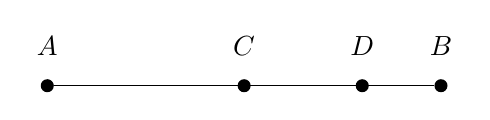
\begin{tikzpicture}
\node[fill,circle,scale=0.5] (a) at (0,0){};
\node[fill,circle,scale=0.5] (c) at (2.5,0){};
\node[fill,circle,scale=0.5] (d) at (4,0){};
\node[fill,circle,scale=0.5] (b) at (5,0){};
\draw (a) -- (b);
\node at (0,0.5){$A$};
\node at (2.5,0.5){$C$};
\node at (4,0.5){$D$};
\node at (5,0.5){$B$};
\end{tikzpicture}
\end{center}

\vspace{.2in}

If $AC=x,$ $CD=y$ and $DB=z$, rewrite the proposition using the symbols $x$, $y$, and $z$ and modern algebraic notation. Then show that this algebraic relationship is true.\\

Translation: Given that $x=y+z$, it follows that $(x+y)^2+z^2=2(x^2+y^2)$.\\

Demonstration of Correctness:\\
Using the assumption that $x=y+z$, we know $z=x-y.$\\
We need to show that $(x+y)^2+z^2=2(x^2+y^2),$ so first we replace $z$ with $x-y$ to obtain:\\

$(x+y)^2+(x-y)^2=2(x^2+y^2)$.\\

Now, we multiply out the left-hand side and collect terms until it looks like the right-hand side of the equation.\\

$(x+y)^2+(x-y)^2=x^2+2xy+y^2+x^2-2xy+y^2=2x^2+2y^2=2(x^2+y^2($

\ee
\end{document}
%%%%%%%%%%%%%%%%%%%%%%%%%%
%%%%%%%END
%%%%%%%%%%%%%%%%%%%%%%%%%%


 